\documentclass[main.tex]{subfiles}

\begin{document}

\section{Summary}
\label{sec:summary}
   
This project was developed for to the curricular course RCOM (Computer Networks).
It was finished successfully by implementing all the required functionalities, passing all the tests, and building a fully working application, with more options, functionalities and high robustness to errors.

The main conclusion to take from this project is the convenience of implementing a communication protocol with a layered architecture, which allows for technical implementation details, hardware configuration and transmission errors to be abstracted from practical applications.

% This section needs a lot of work.
\section{Introduction}
\label{sec:intro}

This program’s goal is to transfer files from one computer to another through a serial port connection, using a \emph{Step and Wait} protocol made with two layers: the \emph{Link Layer}, immediately above the physical layer, whose function is to detect and correct transmission errors and regulate data flow; and the \emph{Application Layer}, handling packets transmission through the link layer. The protocol to implement has a specification described in detail, which we will not reiterate here.

To build the program simply call \plaincode{make} in the main directory. Afterwards, call \plaincode{./ll ----help}. Some use cases can be found in \autoref{subsec:callusecases}.

\subsection{Quick rundown}
\label{subsec:rundown}

\begin{tabular}{ll}
	\nameref{sec:arch} & Architectural aspects, bottom up \\
	\nameref{sec:usecases} & Top down function call tree, example program invocations \\
	\nameref{sec:llprotocol} & Link layer requirements, subunits and sample code \\
	\nameref{sec:alprotocol} & App layer requirements and sample code \\
	\nameref{sec:validation} & Description of tests performed \\
	\nameref{sec:pefficiency} & Program practical vs theoretical efficiency analysis
\end{tabular}

\subsection{Concepts}
\label{subsec:concepts}

We'll use the following labels a few times throughout the report:

\begin{tabular}{lp{0.8\textwidth}}
$LL$ & The Link Layer\\
$AL$ & The Application Layer\\
$R$ & The Receiver (in a program call)\\
$T$ & The Transmitter (in a program call)\\
$TLV$ & A tuple (\var{Type},\var{Length},\var{Value}) used in control packets of the app layer to store information, namely filesize and filename
\end{tabular}

\section{Architecture}
\label{sec:arch}

In this section we will traverse \textit{bottom-up} the program's architectural aspects, including the internal and auxiliary functions of each layer, their interfaces and the primary data structures used. At the end we list some of the auxiliary features such as terminal setup, program options, signal handlers and execution timing.

\subsection{String}
\label{subsec:string}

Given that the byte arrays used throughout the program are \emph{not} \nullp-terminated strings --- but rather of variable length and dynamically allocated --- they must be \textit{accompanied} by their size anytime they are passed between functions. The \struct{string} structure is a simple wrapper around a \struct{char*} and a \struct{size_t}.

\subsection{Link Layer}
\label{subsec:llarch}

The link layer contains one fundamental, yet simple data structure: \struct{frame}. It holds information both for the frame's header ($A$ and $C$ fields) and the frame's data field, which is a \struct{string}.

\subsubsection{Functions}
\label{subsubsec:funcllarch}

The core has the following functionalities and respective functions:

\begin{itemize}[noitemsep,rightmargin=3em]
\item Byte stuffing and destuffing:
\function{stuffData}, \function{destuffData}, \function{destuffText}

\item Convert a \struct{frame} to a \struct{string} and write it to the device:
\function{buildText}, \function{writeFrame}

\item Read text from the device and convert it to a \struct{frame}:
\function{readText}, \function{readFrame}

\item Introduce flip bits in read frames with a certain probability: \function{introduceErrors}
\end{itemize}

On top of these, we have simple utility functions used by the interface:

\begin{itemize}[noitemsep,rightmargin=3em]
\item Inquire frames: \function{is*frame} ---
\function{isIframe}, \function{isSETframe}, \textellipsis

\item Write frames: \function{write*frame} ---
\function{writeIframe}, \function{writeSETframe}, \textellipsis
\end{itemize}

And the interface follows the specification:

\begin{itemize}[noitemsep,rightmargin=3em]
\item Establish a connection through an open device:
\function{llopen}

\item Terminate a connection through an open device:
\function{llclose}

\item Write a message (frame):
\function{llwrite}

\item Read a message (frame):
\function{llread}
\end{itemize}

It should be noted that \function{llopen} and \function{llclose} \emph{do not} open or close the device, nor do they modify any terminal settings.

\subsection{App Layer}
\label{subsec:alarch}

The app-layer makes public three data structures: \struct{tlv}, \struct{control_packet} and \struct{data_packet}. \struct{control_packet} holds an array of \struct{tlv}s, which are the $TLV$ tuples described in the introduction. The \struct{data_packet} structure holds the data of both the packet's header and data field, which is a \struct{string}.

\subsubsection{Functions}
\label{subsubsec:funcalarch}

The app-layer core has the following internal functions:

\begin{itemize}[noitemsep,rightmargin=3em]
\item Convert integers and strings to \struct{tlv}s:
\function{build_tlv_str}, \function{build_tlv_uint}

\item Convert a generic array of \struct{tlv}s to a \struct{control_packet}:
\function{build_control_packet}

\item Convert a \struct{string} to a \struct{data_packet}:
\function{build_data_packet}

\item Extract any \struct{tlv} value from a \struct{control_packet}:
\function{get_tlv}

\item Inquire packets:
\function{isDATApacket}, \function{isSTARTpacket}, \function{isENDpacket}
\end{itemize}

The interface provided to the application user includes:

\begin{itemize}[noitemsep,rightmargin=3em]
\item Send packets using \function{llwrite}:
\function{send_data_packet}, \function{send_start_packet}, \function{send_end_packet}

\item Receive (any) packet using \function{llread}:
\function{receive_packet}

\item Extract filename and filesize from a \struct{control_packet}:
\function{get_tlv_filesize}, \function{get_tlv_filename}
\end{itemize}

\subsection{Parallel features}
\label{subsec:parallelarch}

\begin{itemize}[noitemsep,rightmargin=3em]
\item Open chosen device and set new terminal settings:
\function{setup_link_layer}

\item Close chosen device and set old terminal settings:
\function{reset_link_layer}

\item Alarm utilities for write timeouts:
\function{set_alarm}, \function{unset_alarm}, \function{was_alarmed}

\item Execution timing:
\function{begin_timing}, \function{end_timing}, \function{await_timeout}

\item Compute and print statistics about error probabilities, speed and efficiency:
\function{print_stats}

\item File I/O entry functions:
\function{receive_file}, \function{send_file}, \function{receive_files}, \function{send_files}
\end{itemize}

\section{Use cases and control flow}
\label{sec:usecases}

\subsection{Top level}
\label{subsec:topusecases}

Setup in function \function{main} includes parsing and validating program options with \function{parse_args}, setting up signal handlers with \function{set_signal_handlers}, testing the system's alarms with \function{test_alarm}, and adjusting the terminal configuration with \function{setup_link_layer}.
This is identical for $R$ and for $T$.

In function \function{send_file}, called by $T$, the selected file is opened, its size is calculated and it is then read into a single \emph{buffer} and closed.
The \emph{buffer} is then split into multiple \emph{packets} with length \var{packetsize} --- each stored in a \struct{string} --- and then freed.
These packets are then sent to $R$ in the communications phase, each in its own data packet --- see \autoref{fig:al-transmitter}.

Function \function{receive_file}, called by $R$, enters the communications phase immediately --- see \autoref{fig:al-receiver}.
Once the transmission is completed, it has received a filename and several packet strings.
The output file is created with that filename, the packets are written successively, and then it is closed.

Neither of these functions deal with any $LL$ or internal $AL$ errors. The only errors that may surface are timeout and write retries being capped due to too many errors (see options \plaincode{----time}, \plaincode{----answer} and \plaincode{----timeout}).
At the end of \function{main}, the terminal settings are reset with \function{reset_link_layer}.

\subsection{Calling the program}
\label{subsec:callusecases}

\begin{itemize}[noitemsep,rightmargin=3em]
	\item Transmitter:\\
	\plaincode{./ll -t [option...] files...}
	\item Receiver:\\
	\plaincode{./ll -r [option...] number_of_files}
\end{itemize}

The program supports the usual \plaincode{----help}, \plaincode{----usage} and \plaincode{----version} options. The first two will present all the other possible options and exit.

The program is usually called with just one file, so the only positional argument for $T$ is the name of the file --- which will be used as output filename for $R$. The only position argument for $R$ is the number of files to be received, usually $1$. Multiple files are sent in succession, one after another.

Some example calls:

\begin{itemize}[noitemsep,rightmargin=3em]
	\item Send \file{penguin.png}. In $R$, introduce errors both in frames' headers and data fields:\\
	\plaincode{./ll -t ----stats penguin.png}\\
	\plaincode{./ll -r ----stats -h 0.4 -f 0.6 1}
	\item Calls made for the statistics in \autoref{fig:statistics-f}, with \texttt{ERRORP} $\in\{0,0.2,\ldots,0.97\}$:\\
	\plaincode{./ll -t -s 2048 -b 38400 ----compact ----timeout=5 ----answer=3000 ~/img/landscape.jpg}\\
	\plaincode{./ll -r -s 2048 -b 38400 ----compact ----timeout=5 ----answer=3000 1 -f ERRORP}\\
\end{itemize}

\begin{figure}[ph]
\caption{Sequence diagrams of some important functions\label{fig:seqdiagrams}}
	
\begin{minipage}{0.5\textwidth}
\centering
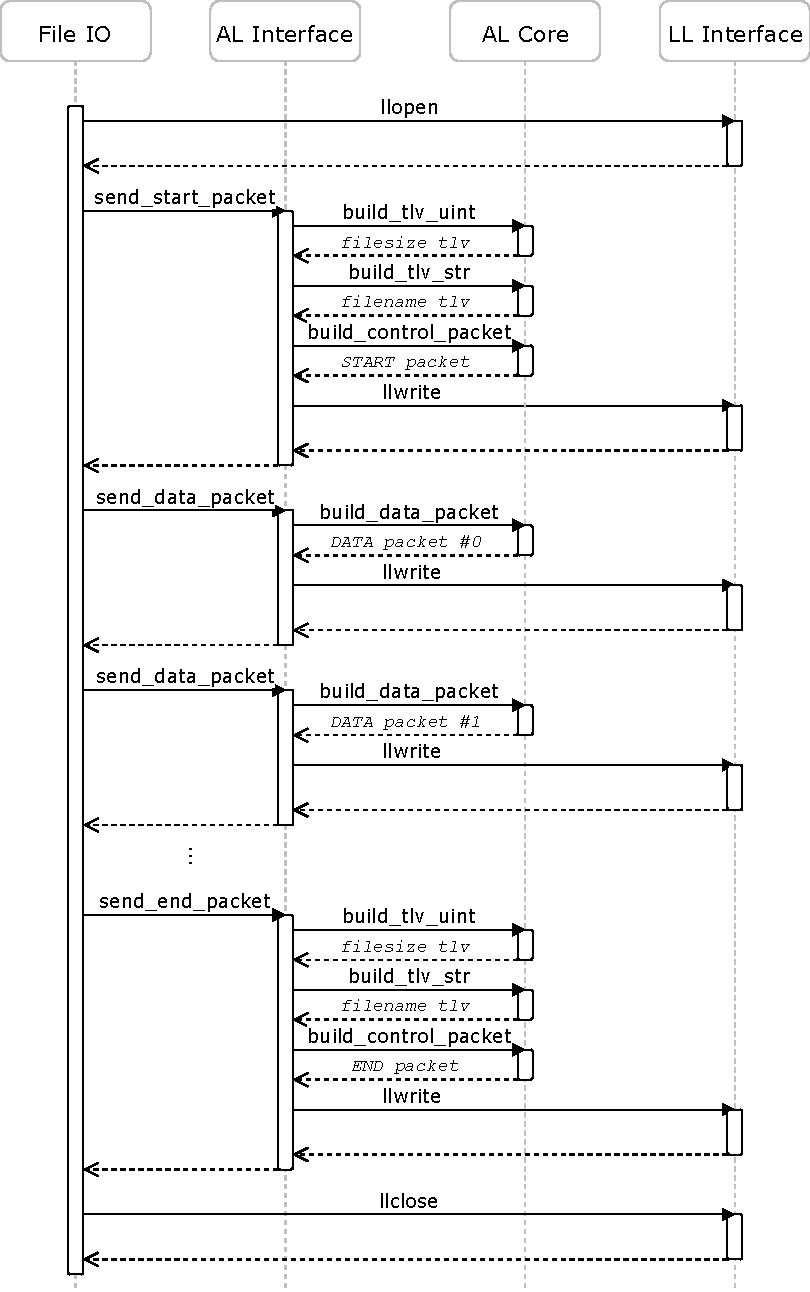
\includegraphics[scale=0.45]{rcom-al-transmitter.pdf}
\subcaption{File communications as seen through the app layer (part of function \function{send_file})\label{fig:al-transmitter}}
\end{minipage}
\begin{minipage}{0.5\textwidth}
\centering
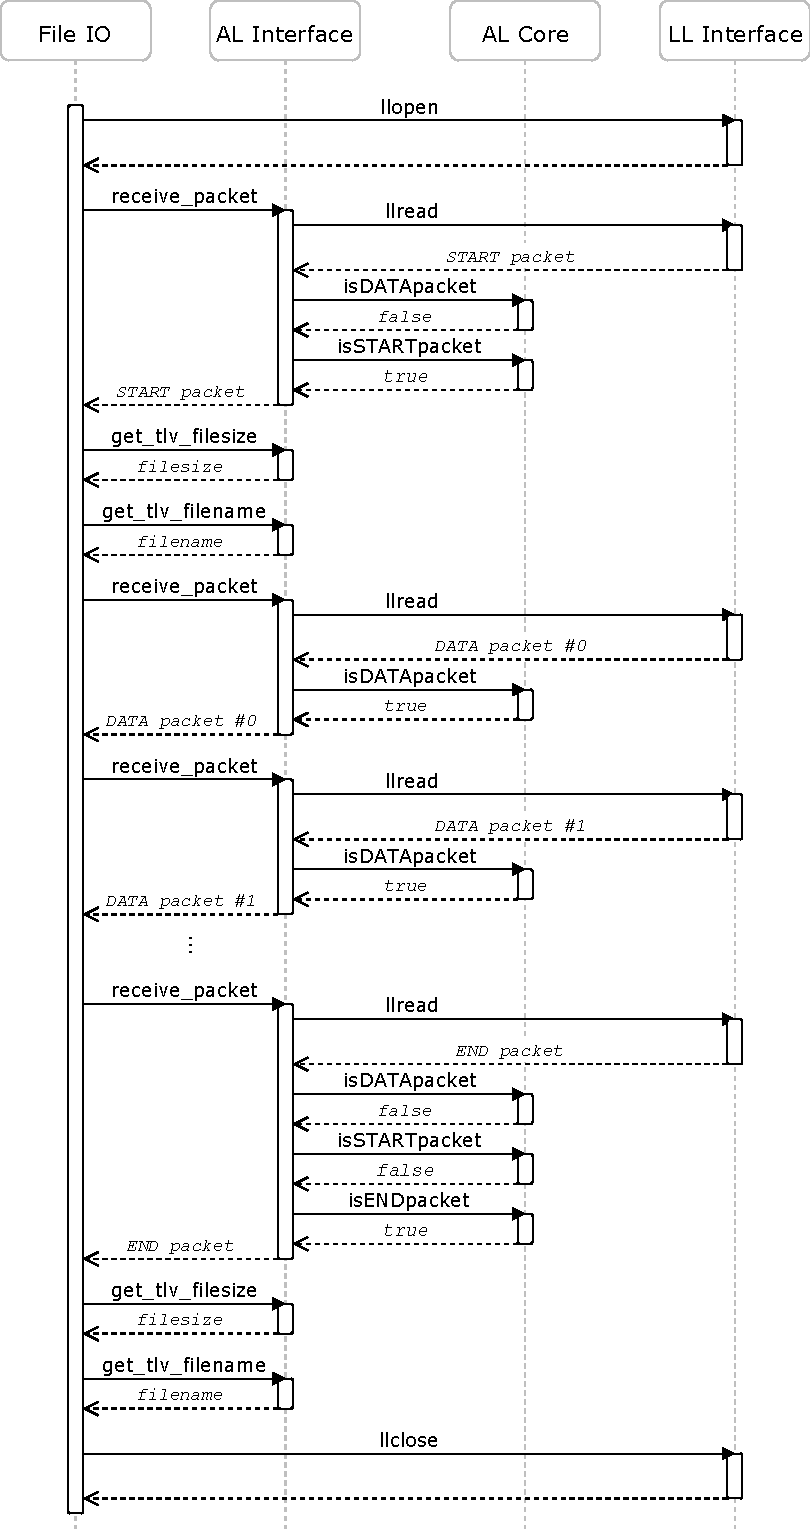
\includegraphics[scale=0.45]{rcom-al-receiver.pdf}
\subcaption{File communications as seen through the app layer (part of function \function{receive_file})\label{fig:al-receiver}}
\end{minipage}
\begin{minipage}{0.5\textwidth}
\centering
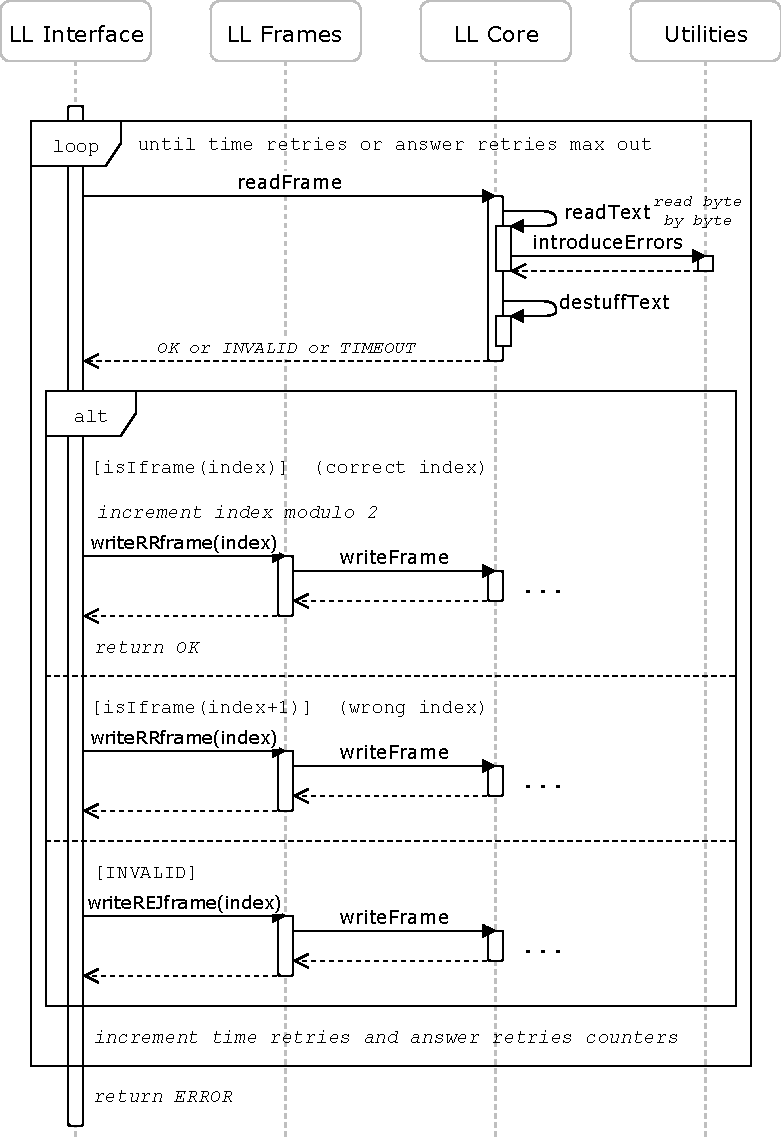
\includegraphics[scale=0.45]{rcom-llread.pdf}
\subcaption{Function \function{llread}\label{fig:llread}}
\end{minipage}
\begin{minipage}{0.5\textwidth}
\centering
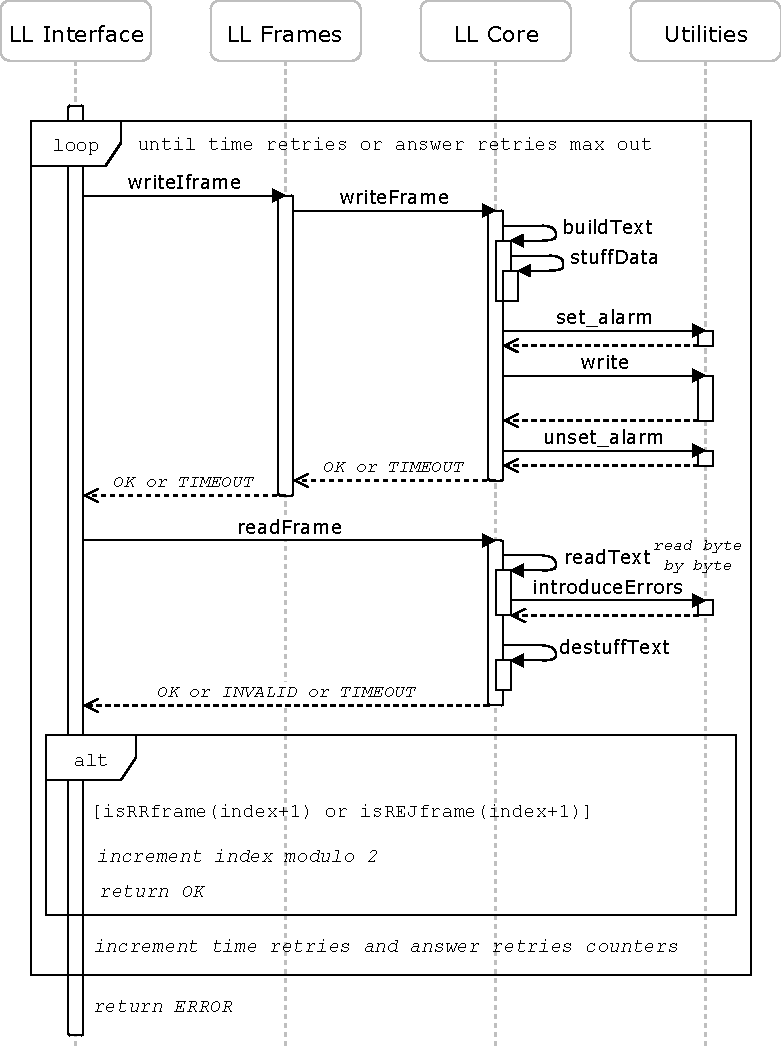
\includegraphics[scale=0.45]{rcom-llwrite.pdf}
\subcaption{Function \function{llwrite}\label{fig:llwrite}}
\end{minipage}
\end{figure}

\section{Link Layer Protocol}
\label{sec:llprotocol}

\begin{wrapfigure}[40]{r}[1.2cm]{0.41\textwidth}
\begin{lstlisting}[style=rcom]
static int readText(int fd, string* textp) {
	string text;
	
	text.len = 0;
	text.s = malloc(8 * sizeof(char));
	
	size_t reserved = 8;
	FrameReadState state = READ_PRE_FRAME;
	int timed = 0;
	
	while (state != READ_END_FLAG) {
		char readbuf[2];
		ssize_t s = read(fd, readbuf, 1);
		char c = readbuf[0];
		
		// [...] Errors and text.s realloc

		switch (state) {
		case READ_PRE_FRAME:
			if (c == FRAME_FLAG) {
				state = READ_START_FLAG;
				text.s[text.len++] = FRAME_FLAG;
			}
			break;
		case READ_START_FLAG:
			if (c != FRAME_FLAG) {
				if (FRAME_VALID_A(c)) {
					state = READ_WITHIN_FRAME;
					text.s[text.len++] = c;
				} else {
					state = READ_PRE_FRAME;
					text.len = 0;
				}
			}
			break;
		case READ_WITHIN_FRAME:
			if (c == FRAME_FLAG) {
				state = READ_END_FLAG;
				text.s[text.len++] = FRAME_FLAG;
			} else {
				text.s[text.len++] = c;
			}
			break;
		default:
			break;
		}
	}

	text.s[text.len] = '\0';
	
	introduceErrors(text);
	
	*textp = text;
	return 0;
}



int writeFrame(int fd, frame f) {
	string text;
	buildText(f, &text);
	
	set_alarm();
	errno = 0;
	ssize_t s = write(fd, text.s, text.len);
	
	int err = errno;
	bool b = was_alarmed();
	unset_alarm();
	
	free(text.s);
	
	if (b || err == EINTR) {
		// [...] Report error
		return FRAME_WRITE_TIMEOUT;
	} else {
		return FRAME_WRITE_OK;
	}
}
\end{lstlisting}
\end{wrapfigure}

In the $LL$ protocol we recognize these requirements:

\begin{enumerate}[label=(\alph*),noitemsep,rightmargin=3em]
\item Canonical, state machine based reading loop of variable length byte arrays;
\item Timeout in long reads and writes;
\item Conversions between byte arrays and a generic frame data structure;
\item Stuffing and destuffing byte arrays, representing valid or invalid generic frames;
\item Error detection and reporting in read frames;
\item Probability based error introduction in read frames;
\item Identification and writing of protocol-defined frames.
\end{enumerate}

Our $LL$ implementation consists of four units: \emph{core}, \emph{errors}, \emph{frames} and \emph{interface}.

\paragraph{Core}
The lowest unit of the entire program, it handles the first five requirements.
Internally it uses mostly \struct{string} instead of \struct{frame}, both for reading and writing.
It exposes only \function{writeFrame} and \function{readFrame}, which have \struct{frame} arguments.
Function \function{writeFrame} calls \function{buildText} to transform the given \struct{frame} into a string, which is \textit{stuffed} by \function{stuffData} before being written.
Function \function{readFrame} calls \function{readText}, the canonical read loop, and destuffs the string read with \function{destuffText}, while validating it and reporting on any detected errors.

This unit supports the entire $LL$ by providing a generic read\slash write facility for frames of any kind --- supporting all valid frame headers and all frame lengths --- by handling only byte stuffing, error detection, and reading/writing timeouts.

\paragraph{Errors}
A simple unit whose purpose is to intentionally introduce errors (bit flips), with a certain probability, in both the header and data fields of frames. Entered at the end of function \function{readText}.

\paragraph{Frames}
For each frame in the specification -- \fI{}, \fSET{}, \fDISC{}, \fUA{}, \fRR{}, and \fREJ{} -- this unit exposes a function which identifies it, \function{is*frame}, and another which writes it to a given file, \function{write*frame}.

\paragraph{Interface}
Includes specified functions \function{llopen}, \function{llwrite}, \function{llread} and \function{llclose}.
These functions use only the facilities provided by the \emph{frames} unit.
\function{llopen} is used to establish a connection between $R$ and $T$ by ensuring both ends are in sync; \function{llclose} is used to end it.
These functions have different \textit{versions} for $R$ and $T$.
While the connection is active, \function{llread} and \function{llwrite} are used to read and write from the connection respectively.

\section{Application Layer Protocol}
\label{sec:alprotocol}

\begin{wrapfigure}[31]{r}[1cm]{0.41\textwidth}
\begin{lstlisting}[style=rcom]
int send_start_packet(int fd, size_t filesize, char* filename) {
	int s;
	string tlvs[2];
	
	out_packet_index = 0;
	
	s = build_tlv_uint(PCONTROL_TYPE_FILESIZE,
	 filesize, tlvs + FILESIZE_TLV_N);
	if (s != 0) return s;
	
	s = build_tlv_str(PCONTROL_TYPE_FILENAME,
	 string_from(filename), tlvs + FILENAME_TLV_N);
	if (s != 0) return s;
	
	string start_packet;
	s = build_control_packet(PCONTROL_START,
	 tlvs, 2, &start_packet);
	if (s != 0) return s;
	
	free(tlvs[0].s);
	free(tlvs[1].s);
	
	// [...] Report app write
	
	s = llwrite(fd, start_packet);
	free(start_packet.s);
	return s;
}



int receive_packet(int fd, data_packet* datap,
	  control_packet* controlp) {
	int s;
	
	string packet;
	s = llread(fd, &packet);
	if (s != 0) return s;
	
	data_packet data;
	control_packet control;
	
	if (isDATApacket(packet, &data)) {
		++in_packet_index;
		*datap = data;
		
		free(packet.s);
		return PRECEIVE_DATA;
	}
	
	if (isSTARTpacket(packet, &control)) {
		in_packet_index = 0;
		*controlp = control;
		
		free(packet.s);
		return PRECEIVE_START;
	}
	
	if (isENDpacket(packet, &control)) {
		in_packet_index = 0;
		*controlp = control;
		
		free(packet.s);
		return PRECEIVE_END;
	}
	
	printf("[APP] Error: Received BAD packet\n");
	free(packet.s);
	return PRECEIVE_BAD_PACKET;
}
\end{lstlisting}
\end{wrapfigure}

In the $AL$ protocol we recognize these requirements:

\begin{enumerate}[label=(\alph*),noitemsep,rightmargin=3em]
\item Representation of generic control packets and data packets;
\item Construction of a control packet from a list of values;
\item Construction of a data packet from a string;
\item Identification, parsin	g and writing of protocol-defined packets;
\item Extraction of \struct{tlv} values from control packets, namely filesize and filename;
\item Error detection and reporting of mis-indexed \pDATA{} packets or bad packets.
\end{enumerate}

Our $AL$ implementation, unlike the $LL$ implementation, is not further subdivided.
Each of these requirements is satisfied by a set of specialized functions, and the interface is essentially \function{send_data_packet}, \function{send_start_packet}, \function{send_end_packet} and \function{receive_packet}.

The first function, \function{send_data_packet}, takes a \struct{string}, prepends it with a packet header using \function{build_data_packet}, and writes it using \function{llwrite}.
The packet index is kept in an internal counter \var{out_packet_index}.
The other functions \function{send_start_packet} and \function{send_end_packet} first build two \struct{tlv} for the filesize and filename using \function{build_tlv_*}, then build the control packet string using \function{build_control_packet}, and finally write it using \function{llwrite}.

The \function{receive_packet} function reads an arbitrary packet using \function{llread}, and then uses \function{isDATApacket}, \function{isSTARTpacket} or \function{isENDpacket} to identify \emph{and} parse said packet.
The packet index is also kept in an internal counter \var{in_packet_index}.

\section{Validation}
\label{sec:validation}

Multiple successive tests were made in order to determine the robustness of the program:

\begin{enumerate}[label=(\alph*),noitemsep,rightmargin=3em]
\item Send a file without errors;
\item Introduce errors in the serial port with pins (RCOM lab);
\item Introduce errors (flip bits) internally, in frames' headers and/or data fields;
\item Turn off and on the connection in the serial port repeatedly, halting communications;
\item All the previous attempt of failures together.
\end{enumerate}

The program is robust to these errors, and only (b) can potently corrupt a frame in an undetectable manner --- due to the weaknesses in the protocol --- resulting in a corrupted output file. For point (c), errors were introduced in control frames's headers as well, corrupting frames \fSET{}, \fDISC{} and \fUA{} used in functions \function{llopen} and \function{llclose}. These succeed regardless, although possibly only after several timeouts. See options \plaincode{-f}, \plaincode{-h}, \plaincode{----time}, \plaincode{----timeout}.

\section{Protocol Efficiency}
\label{sec:pefficiency}

\subsection{Errors in frame data field: Noisy transmission}
\label{subsec:noisy}

To approach this topic, analyze the following chart, \autoref{fig:statistics-f}.

\begin{figure}[htbp]
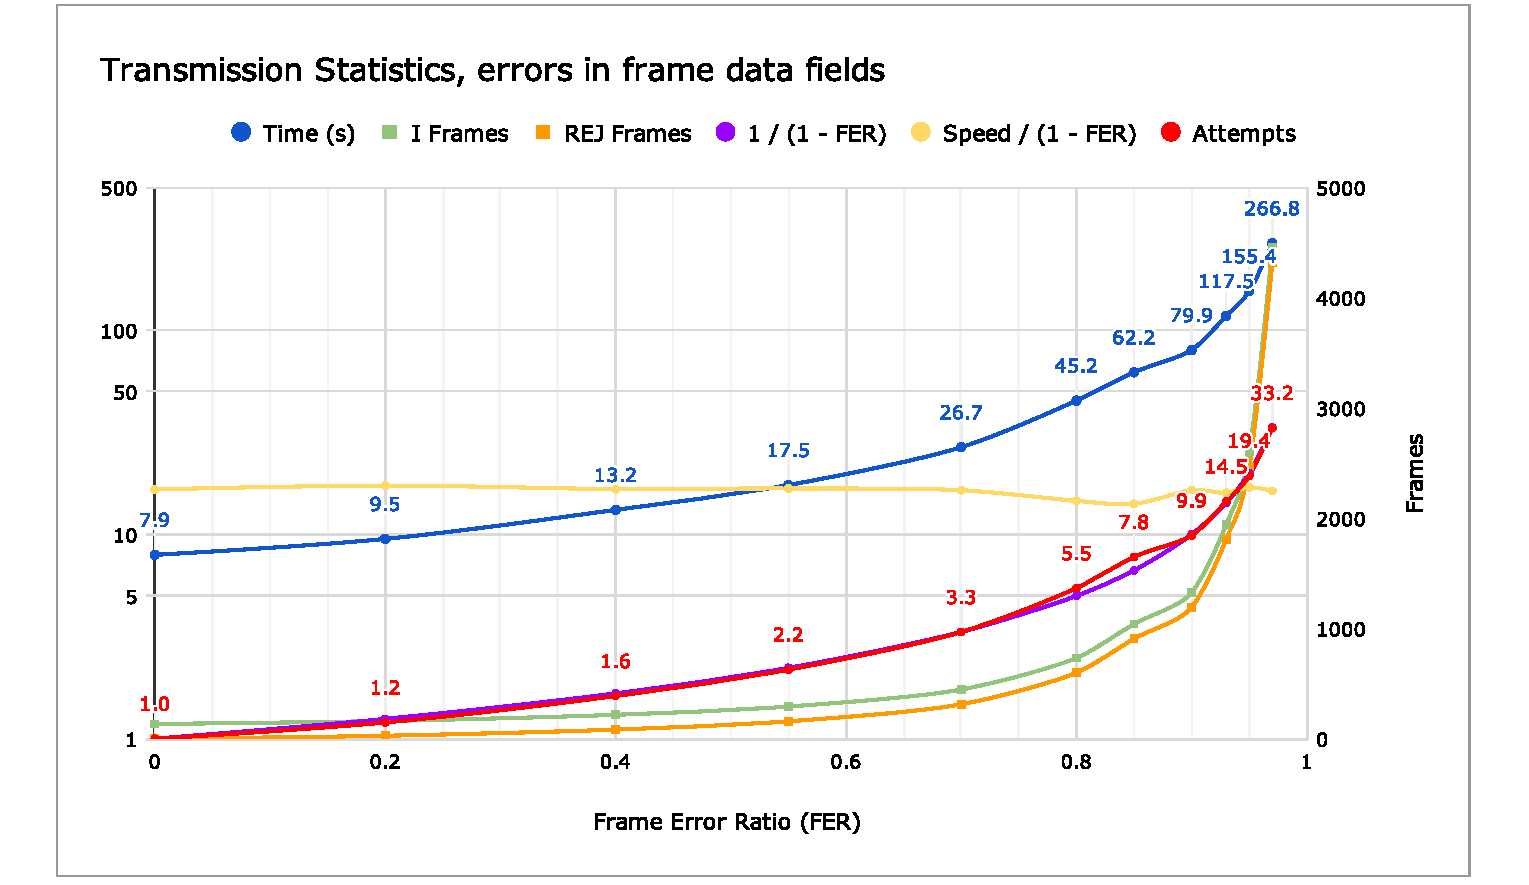
\includegraphics[width=\textwidth]{graph-f.pdf}
\caption{Transmission statistics of a 268.849B file, using packetsize 2048 and baudrate 38400 bytes/s.\\ Error probability samples (\plaincode{-f}): $\texttt{FER}=p\in\{0,0.2,0.4,0.55,0.7,0.8,0.85,0.9,0.93,0.95,0.97\}$.}
\label{fig:statistics-f}
\end{figure}

First of all, with the specified parameters the file is split into 132 packets, with average packet size 2037 and \fI{} frame size 2047 bytes. Since there are no frame header errors, a total of 134 packets is transmitted, and $T$ receives exactly $134$ \fRR{} acknowledgments.

The green and orange graphs count the number of transmitted \fI{} and \fREJ{} frames respectively (right vertical axis). At $p=0.93$, these numbers round 2000. Since the total number of packets is constant, the orange curve is just a translation of the first.

\emph{Attempts} is the graph of $\tfrac{\#\fI}{\#\fRR}=\tfrac{\#\fI}{\#\fI-\#\fREJ}$. This is the average number of times $T$ has to write a frame \fI{} to the device before it is acknowledged by $R$ and received without errors. We can see it follows the graph of $1/(1-\texttt{FER})$, a consequence of the relation

\begin{equation*}
	\mathbb{E}[Attempts] = \sum_k k\cdot \mathbb{P}[Attempts=k] = \sum_k k\cdot p^{k-1}(1-p)=\frac{1}{1-p}.
\end{equation*}

Furthermore, \emph{Speed} is the data packet rate, i.e. the number of packets transmitted per second. Its formula is $\tfrac{\var{filesize}}{2037 \cdot \var{s}}$ --- or in this case simply $\tfrac{132}{\emph{Time}}$. The yellow graph traces $\emph{Speed}/(1-\texttt{FER})$, which is approximately constant --- around 16.2. Indeed, \emph{Speed} is just a scaled measure of \emph{Efficiency}, which in our case is theoretically

\begin{equation*}
	S = \frac{T_f}{\mathbb{E}[A]\cdot(T_f + 2T_{prop})} = \frac{1}{\mathbb{E}[A]\cdot(1+2a)} = \frac{1-p}{1+2a} \stackrel{a=0}{\simeq} 1-p.
\end{equation*}

Finally, with this analysis we can conclude in multiple ways --- the simplest of which just reading the chart --- that the total transmission time is inversely proportional to $\tfrac{1}{1-p}$, i.e. linear in $1-p$.

\subsection{Errors in frame header}
\label{subsec:errheaders}

For completion, we leave here a chart similar to the previous one, with the same parameters expect replacing \var{-f} with \var{-h}, i.e. introducing the errors in the frames' headers instead of data fields.

\begin{figure}[htbp]
	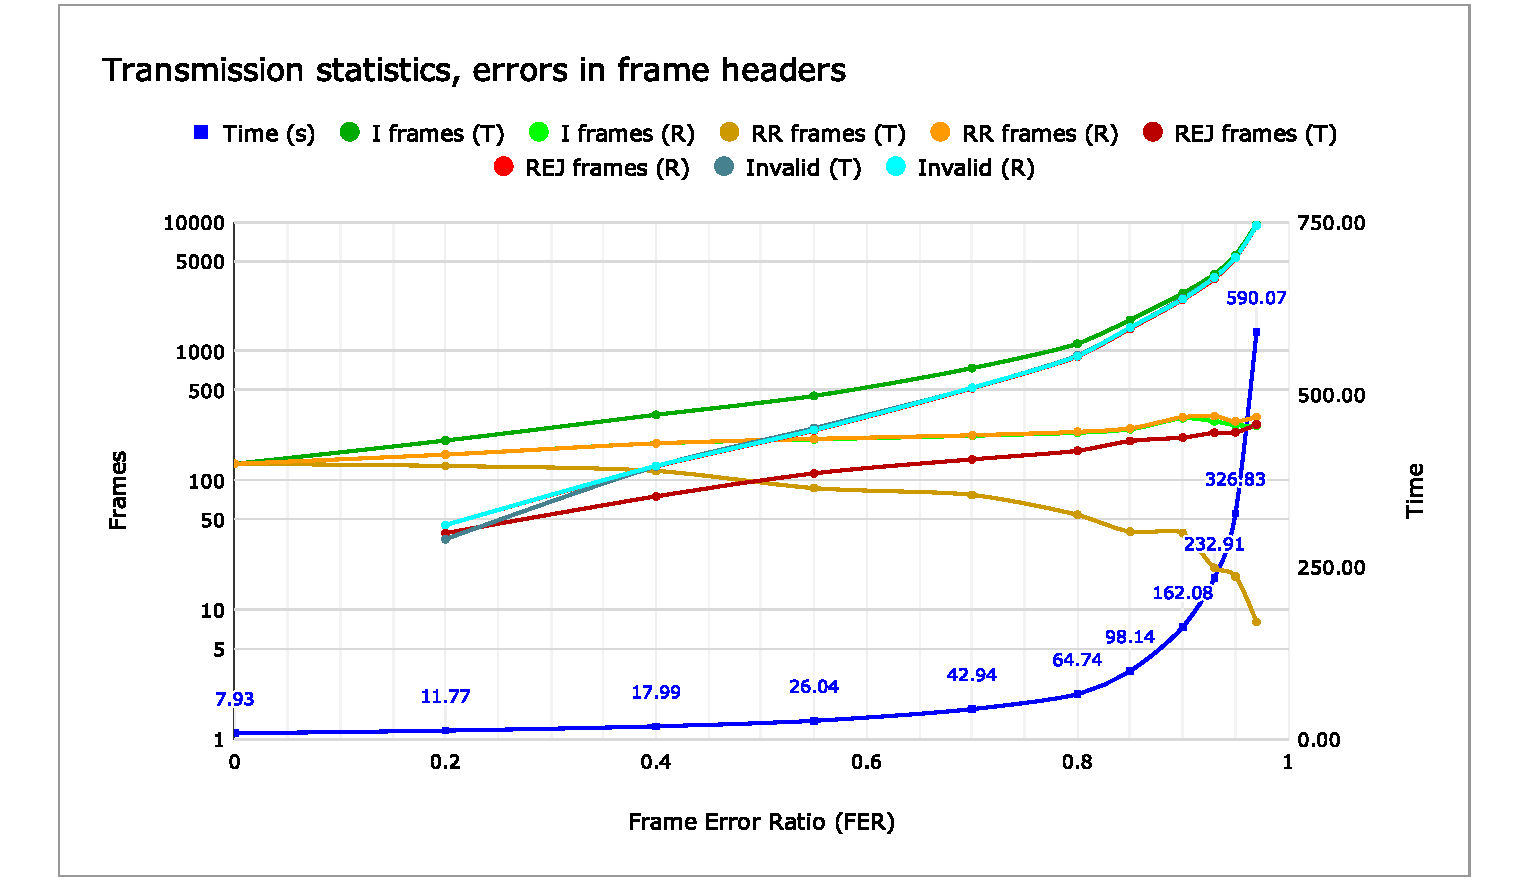
\includegraphics[width=\textwidth]{graph-h.pdf}
	\caption{Transmission statistics of a 268.849B file, using packetsize 2048 and baudrate 38400 bytes/s.\\ Error probability samples (\plaincode{-h}): $\texttt{FER}=p\in\{0,0.2,0.4,0.55,0.7,0.8,0.85,0.9,0.93,0.95,0.97\}$.}
	\label{fig:statistics-h}
\end{figure}

\section{Conclusion}
\label{sec:conclusion}

We implemented all of the specified requirements, and built an implementation of the protocol with multiple configurations, performance analysis and robustness.

The most challenging part in the development phase was implementing \function{llopen} and \function{llclose} in such a way they would succeed even with high error probabilities in frame headers (\var{-h}).

\end{document}
